\documentclass[fontsize=10pt]{article}
\usepackage[utf8]{inputenc}
\usepackage[T1]{fontenc}
\usepackage{graphicx} % handles figures
\usepackage{mathtools}
\usepackage{amsmath}
\usepackage{hyperref}
\usepackage{amssymb}
\usepackage{xcolor}
\usepackage[shortlabels]{enumitem}
%Insertion de tout un tas de librairie qui nous seront probablement inutiles pour la pluspart mais it's always good to have them
\title{\textbf{Maths Discrètes}\\ Solutions TP 6}
\date{}
\begin{document}
\maketitle % fais le titre écris plus haut


\section*{Exercice 1}
\begin{align*}
n &= \frac{mL -1}{m-1}\\
&= \frac{3\times 521 -1}{3-1}\\
&= 781
\end{align*}
\begin{align*}
h &= \lceil log_3(521) \rceil\\
&= \lceil 5.69 \rceil\\
&= 6
\end{align*}
\begin{align*}
i &= \frac{l -1}{m-1}\\
&= \frac{l-1}{2}\\
&= 26
\end{align*}

Comme entier et équilibré, seuls les deux derniers niveaux possèdent des feuilles.
\begin{itemize}
\item $h_5$ possède $i - \underset{k=0}{\overset{4}{\sum}}3^k = 139$ sommets.\\
si $h_5$ n'avait pas de feuilles, il avait $3^5 = 243$ sommets donc $h_5$ possède $243-139 =104$ feuilles.
\item $h_6$ possède donc $521-104$ ou $139 \times 3 = 417$ feuilles.
\end{itemize}


\section*{Exercice 2}


1.\\ 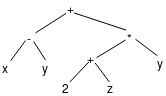
\includegraphics[scale=1]{TP6Exo2_1.jpg} 


\hspace{-0.58cm}2.\\ 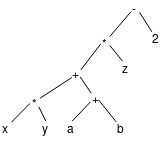
\includegraphics[scale=1]{TP6Exo2_2.jpg} 

\section*{Exercice 3}
\begin{enumerate}
\item * - x y - + x 17 7
\item x y - x 17 + 7 - *
\end{enumerate}

\section*{Exercice 4}
\begin{enumerate}[(a)]
\item 3 arbres sous-tendants
\item 4 arbres sous-tendants
\item 5 arbres sous-tendants
\item 16 arbres sous-tendants
\end{enumerate}

\section*{Exercice 5}
\begin{alignat*}{10}
&a \hspace{1pt}\rule{10pt}{1pt} \hspace{1pt}&&b\hspace{1pt}\rule{10pt}{1pt} \hspace{1pt}&&c\hspace{1pt}\rule{10pt}{1pt}\hspace{1pt} &d\\
& \hspace{1pt}\rule{1pt}{10pt}&&\hspace{1pt}\rule{1pt}{10pt} &&\hspace{1pt}\rule{1pt}{10pt} &\\
&e &&f &&g &h\\
& &&\hspace{1pt}\rule{1pt}{10pt} && &\hspace{1pt}\rule{1pt}{10pt}\\
&i\hspace{1pt}\rule{10pt}{1pt} \hspace{1pt} &&j \hspace{1pt}\rule{10pt}{1pt} \hspace{1pt}&&k\hspace{1pt}\rule{10pt}{1pt} \hspace{1pt} &l
\end{alignat*}

\section*{Exercice 6}
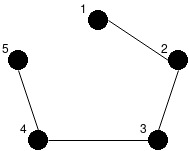
\includegraphics[scale=1]{TP6Exo5.jpg} 

\section*{Exercice 7}
Même principe que TP 4 exercice 5.

\section*{Exercice 8}
\begin{alignat*}{5}
\underset{k=0}{\overset{n}{\sum}} \hspace{0.1cm}2^k\begin{pmatrix} n \\k\end{pmatrix} &= \underset{k=0}{\overset{n}{\sum}} \begin{pmatrix} n \\k\end{pmatrix} 2^k 1^{n-k}\\
&=(2+1)^n\\
&=3^n
\end{alignat*}

\section*{Exercice 9}

$\underset{k=m}{\overset{n}{\sum}}\hspace{0.1cm}\begin{pmatrix} k\\m\end{pmatrix}\begin{pmatrix} n\\k\end{pmatrix} = 2^{n-m}\begin{pmatrix} n\\m\end{pmatrix}$\\
le nombre de façons de choisir $m$ parmi $k$, et $k$ parmi $n$ soit : \\
le nombre de façons de choisir $m$ parmi $n$ 
($\begin{pmatrix}
n\\
m
\end{pmatrix}$)
 et d'inclure ou non un élément de $n$ dans $k$ ($2^n$), $m$ y étant par définition donc sans choix ($n-m$).\\
\textit{Il existe une solution algébrique, mais même moi qui les préfère en général, je vous dit: ça n'en vaut pas la peine. Mais je l'ai dans mes feuilles si vous êtes curieux.}\\

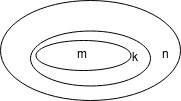
\includegraphics[scale=1]{TP6Exo9.jpg} 

\section*{Exercice 10}
Pour\\$x_1 = \#1$, $x_2 = \#2$,\dots, $x_6 = \#6$ \hspace{1cm} $x_i \geq \in \mathbb{N}$ \\
où $x_i =$ le nombre de dés qui tombent sur la valeur $i$.\\
Si on les additionne tous, on a toujours le nombre de dés qu'on a lancé:\\
$x_1 + x_2 +x_3 + \dots + x_6 =n$\\
On peut donc utiliser un coefficient multinomial.






\end{document}
